\documentclass{article}

% if you need to pass options to natbib, use, e.g.:
%     \PassOptionsToPackage{numbers, compress}{natbib}
% before loading neurips_2020

% ready for submission
% \usepackage{neurips_2020}

% to compile a preprint version, e.g., for submission to arXiv, add add the
% [preprint] option:
    \usepackage[preprint]{neurips_2020}

% to compile a camera-ready version, add the [final] option, e.g.:
%     \usepackage[final]{neurips_2020}

% to avoid loading the natbib package, add option nonatbib:
     % \usepackage[natbib]{neurips_2020}

\usepackage[utf8]{inputenc} % allow utf-8 input
\usepackage[T1]{fontenc}    % use 8-bit T1 fonts
\usepackage{hyperref}       % hyperlinks
\usepackage{url}            % simple URL typesetting
\usepackage{booktabs}       % professional-quality tables
\usepackage{amsfonts}       % blackboard math symbols
\usepackage{nicefrac}       % compact symbols for 1/2, etc.
\usepackage{microtype}      % microtypography
\usepackage{algorithm}
\usepackage{algorithmic}
\usepackage{mathtools}
\usepackage{graphicx}  % allows inclusion of PDF, PNG and JPG images


\newlength\myindent
\setlength\myindent{2em}
\newcommand\bindent{%
  \begingroup
  \setlength{\itemindent}{\myindent}
  \addtolength{\algorithmicindent}{\myindent}
}
\newcommand\eindent{\endgroup}


\bibliographystyle{unsrt}

\title{FedExP in Flower}

% The \author macro works with any number of authors. There are two commands
% used to separate the names and addresses of multiple authors: \And and \AND.
%
% Using \And between authors leaves it to LaTeX to determine where to break the
% lines. Using \AND forces a line break at that point. So, if LaTeX puts 3 of 4
% authors names on the first line, and the last on the second line, try using
% \AND instead of \And before the third author name.

\author{%
  Henry Batchelor\\
  \texttt{htb27@cam.ac.uk} \\
  % examples of more authors
  % \And
  % Coauthor \\
  % Affiliation \\
  % Address \\
  % \texttt{email} \\
  % \AND
  % Coauthor \\
  % Affiliation \\
  % Address \\
  % \texttt{email} \\
  % \And
  % Coauthor \\
  % Affiliation \\
  % Address \\
  % \texttt{email} \\
  % \And
  % Coauthor \\
  % Affiliation \\
  % Address \\
  % \texttt{email} \\
}

\begin{document}

\maketitle

\begin{abstract}
  The goal of this project was to implement the FedExP algorithm as described in \cite{FedExP}, which aims to improve the performance over FedAvg by dynamically altering the server step size, inside of Flower \cite{flower} a framework for Federated Learning.  The secondary aim was to provide an analysis of the algorithm's performance against other algorithms.
\end{abstract}

\section{Problem formulation and preliminaries}

Federated Averaging is a popular method for performing Federated Learning because it is simple to implement, requires minimal communication, statelessness, and ease to add on privacy preservation.  However FedAvg suffers from problems caused by client heterogeneity, which is an intrinsic part of real Federated Learning systems.  It has been shown in recent papers \cite{FewerClientsWorseBehaviour} that this is made worse when only selecting a subset of the total clients which are available for training, which means that in a cross-device setting it can cause significantly more issues, this is also caused by sampling biases in reality of which clients are available to us.  There have been several techniques proposed to deal with these issues, such as in \cite{signSGD} and \cite{ProxSkip}, however each of these have significant drawbacks such as making the clients stateful, adding extra computation, or limiting privacy which are some of the main reason why we want to perform Federated Averaging in the first place.  

Recently this slowdown has been addressed by adding a server learning rate, which controls the step size used when aggregating pseudo-gradients from the clients. \cite{AdaptiveFederatedOptimisation}  For these to work well it is proposed that the client step size is O($\frac{1}{\tau\sqrt{T}}$) and server step size is O($\tau\sqrt{M}$), where $\tau$ is the number of local epochs, $T$ is the number of communication rounds, and $M$ is the number of clients.  In practice however these do not lead to great results because the small client step size impacts the speed of training heavily, which the large global step size cannot be fully compensated for by a large server step size, this is most prevalent in the initial rounds.

FedExP attempts to dynamically set the size of the global step size to ensure fast convergence of the overall model while still having a moderate client step size, it also wants to take into account the heterogeneity between the local objective functions because it has been shown that it can be beneficial to have a smaller server step size if the local objectives differ significantly. \cite{smallServerStepSizeForHetrogeneity}  FedExP accomplishes this by establishing a connection between FedAvg and the Projection Onto Convex Sets (POCS) algorithm.  Using an analogy between the server step size and the extrapolation parameter used to speed up POCS \cite{ExtrapolatedPOCS}, this then allows the new extensions to the algorithm deal with inexact and noisy projections, the main one of interest to us is a time-varying bound on the progress of clients towards the optimal solution and how this can be used to dynamically estimate a good server step size, resulting in FedExP.  These connections and analogies are only strictly valid in the case that the model is over-parameterised, there are more parameters than data points across all clients, this can often be the case with deep neural models.

\begin{algorithm}
\caption{FedExP}
\begin{algorithmic} 
\STATE \textbf{Input:} $\textbf{w}^{(0)}$, number of rounds $T$, local iteration step $\tau$, parameters $\eta_l, \epsilon$\\
\FOR{$t = 0, \ldots, T - 1$ \textbf{communication rounds}}
    \STATE \textbf{Global server does:}
    \STATE Send $\textbf{w}^{(t)}$ to all clients
    \STATE \textbf{Clients} $i \in [M]$ \textbf{in parallel do:}
    \bindent
    \STATE Set $\textbf{w}_i^{(t,0)} \leftarrow \textbf{w}^{(t,0)}$    \FOR{$k = 0, \ldots, \tau - 1$ \textbf{local iterations}}
            \STATE Update $\textbf{w}_i^{(t,k+1)} \leftarrow \textbf{w}_i^{(t,k)} - \eta_l \nabla F_i (\textbf{w}_i^{(t,k)}, \xi_i^{(t,k)})$
        \ENDFOR
        \STATE Send $\Delta_i^{(t)} \leftarrow \textbf{w}^{(t)} - \textbf{w}_i^{(t,\tau)}$
    \eindent
    \STATE \textbf{Global server does:}
    \bindent
    \STATE $\bar{\Delta}^{(t)} \leftarrow \frac{1}{M} \sum_{i=1}^{M}{\Delta_i^{(t)}}$
    \STATE $\eta_g^{(t)} \leftarrow \max\{1, \sum_{i=1}^{M}{\frac{{\lVert\Delta_i^{(t)}\rVert}^2}{2M({\lVert\bar{\Delta}^{(t)}\rVert}^{2} + \epsilon)}}\}$
    \STATE Update global model with $\textbf{w}^{(t+1)} \leftarrow \textbf{w}^{(t)} - \eta_g^{(t)}\bar{\Delta}^{(t)}$
    \eindent
\ENDFOR
\end{algorithmic}

\end{algorithm}

A detail explanation of the derivation and proof of convergence bounds of the FedExP algorithm can be found in \cite{FedExP}.  That being said a couple of the key features will be explained below:

\begin{description}
\item[Need for $\epsilon$]{This has the purpose of ensuring that in later rounds an incredibly large global learning rate is not used.  This is potentially a concern because in later rounds of training it is likely that the overall update applied to the model will be very small but the individual client updates will be significantly larger, therefore if this occurred a very large global learning rate can be achieved which would lead to a significant decrease in performance.  To solve this issue a small value $\epsilon$ is added this ensures that when the updates become small we will have a much greater chance of following FedAvg or still have a reasonable global learning rate.  It should also be said that the value of $\epsilon$ determines the amount of blending between our adaptive strategy and FedAvg, because as $\epsilon$ tends to infinity the algorithm becomes FedAvg (because the max will ensure the global learning rate is always 1).}

\item[Compatibility with Partial Client Participation and Secure Aggregation]{FedExP can be easily modified to support partial client participation in any round by simply only taking the number of participating clients in the steps after we have received updates from the clients in any particular round.  It will also continue to work with Secure Aggregation due to only needing to estimate average of pseudo-gradient norms therefore the changes Secure Aggregation makes to the gradients are possible to be managed.}

\item[FedExP monotonically decreasing ${\lVert\textbf{w}^{(t)} - \textbf{w}^*\rVert}^2$ but not necessarily $F(\textbf{w}^{(t)}) - F(\textbf{w}^*)$]{This is telling us that after every round the distance between the weights and the optimal set of weights will decrease however it is not the case that this means that objective function must also decrease.  This behaviour can also lead to oscillations in the performance of the model as rounds progress because we are bouncing between different paths getting us closer to the optimal set of weights but each of those paths can have quite a lot worse performance than another set of weights a similar distance or further away from the optimal set of weights, this is caused by the differing local objective functions.  This is the main motivation behind averaging out the last n number of rounds of weights returned by FedExP when performing evaluation because it dramatically reduces the degree of the oscillations and can result in better performance by following a lower global loss region.}

\end{description}


\section{Implementation}

\subsection{Strategy}

The strategy which is implemented inside of Flower for this project does not strictly follow the FedExP algorithm described above, because that requires that clients submit their local pseudo-gradients instead of their updated set of weights.  This means that if it was implemented in this manner then the standard Flower clients which can easily be used with other already implemented strategies such as FedAvg, FedAdam, FedYogi etc. would not work due them returning the updated weights.  To allow interoperability with these clients, allowing easier comparison between different strategies because it is possible to isolate that the only change must have been made to the strategy, the pseudo-gradients are instead calculated on the server-side -- this is done by the strategy subtracting off the original set of weights from each of the returned set of weights of each client before carrying on with the computation.

The strategy implemented in Flower also takes as a hyper-parameter the number of rounds which the weights will be averaged over before evaluating the performance of the model, it is suggested in the paper that it can be allowed to have this as a hyper-parameter but that they have it set to 2 for all their experiments.  Having it as a hyper-parameter allows easier experimentation to see how it affects the performance of different models and in different scenarios, for example in certain situations it might be very important to have a smooth training curve (maybe because you are wanting to use the model part way through training, therefore you do not want the performance to suddenly decrease) in which case you will likely want to average over significantly more rounds, this clearly does not change the weights which are being used in training just when evaluating the model.

The implemented strategy also deals with partial client participation naively because all aggregations are performed only over clients which are successful in returning results to us.  

The implementation of the strategy is based on the already existing FedAvg strategy.  The functions which had to be altered are outlined below

\begin{description}
    \item[initialize\_parameters]{This had to be made to not drop the initial parameters from memory when it is called, this is because on the aggregation of the first round it is required that we have those initial parameters to be able to calculate the pseudo-gradients, and after each round they are updated to be the parameters at the start of that round.}
    \item[aggregate\_fit]{This is where the bulk of the changes are because it is affecting how the parameters are updated.  The main changes are that we now compute the pseudo-gradients for all of the clients which have successfully completed the round of training.  Then an unweighted average of these updates is taken to produce the necessary average update to be used in the process of computing the global learning rate.  The calculation of the global learning rate is implemented very closely to how it is described in the FedExP algorithm presented about to make it very clear what is happening where and how any changes you wish to make to that calculation can be achieved.  After the global learning rate has been calculated it is then used in the manner described in FedExP to update the weights which have been stored, we also need to run all the metric aggregation functions which can have been passed in.  The parameters are also stored into a list containing the last k (specified as the hyper-parameter for number of rounds to average evaluation over) rounds of parameters, to allow the evaluation of the correct set of parameters.}
    \item[evaluate]{This is the global evaluation function, the only change here is to use the average set of parameters from the last k rounds (or as many rounds as their have been if we have not had k rounds) when performing the actual evaluation.}
    \item[configure\_evaluate]{Similar changes to evaluate, this makes it so that the clients use the average of the last k rounds of parameters instead of the latest parameters.}
\end{description}

\subsection{Baseline}

This has all be implemented as a baseline as well which allows easy use of the strategy against certain specified data sets with models to show how the performance of the implementation compares to that of the original paper.  In this case I have implemented 4 different data sets described in the original FedExP paper

\begin{itemize}
    \item Synthetic -- This is a randomly generated data set according to the method specified in \cite{syntheticDatasetGeneration}, where we are performing an over-parameterised linear regression.
    \item FEMNIST -- The EMNIST data set where the federated partitioning is based on the writer of the symbols, for this task we are performing classification using a CNN, the architecture used is described in \cite{AdaptiveFederatedOptimisation} for EMNIST CR task.
    \item CIFAR-10 -- The CIFAR-10 data set, where the partitioning is done using a Dirichlet distribution, and a ResNet-18 model \cite{ResNet} is used for the classification task.
    \item CIFAR-100 -- Similar to CIFAR-10 except using the CIFAR-100 dataset.
\end{itemize}

The implementations of the CIFAR data sets follow very closely what is done in the Adaptive Federated Optimization baseline and the FEMNIST data set part is based around the work performed in the course labs.  In all of these cases though the client which is being used had to be changed away from what is used elsewhere (either in the labs or Adaptive Federated Optimization baseline) due to the original FedExP paper \cite{FedExP} using a weight decay for the optimiser, decreasing the client learning rate on each round, and performing gradient clipping during the local training process.  The client therefore looks for these values in the config which is passed on every training round, where there is a custom function to generate the config passed to them.  The values used inside of the function to generate the config for each round, are specified in the overall config of the baseline.

\begin{figure}
    \centerline{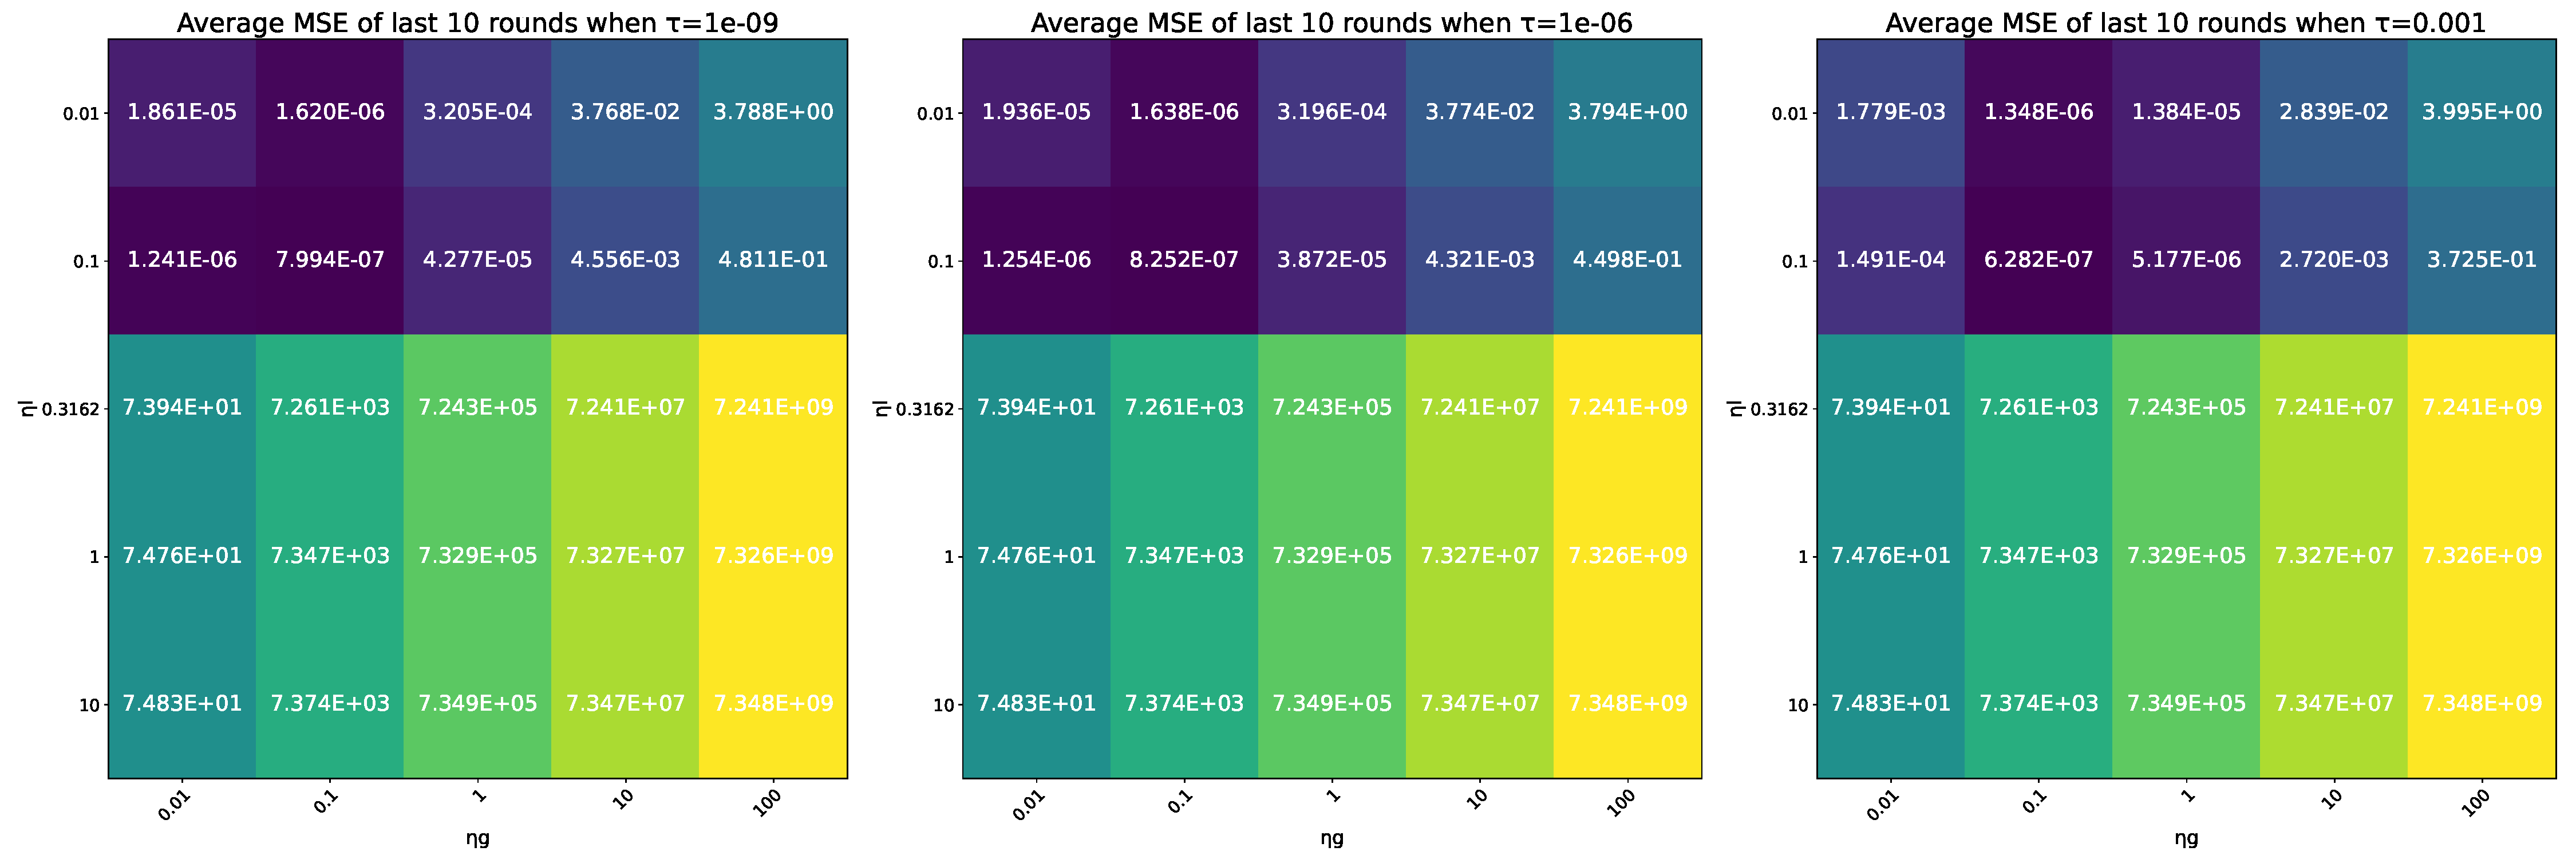
\includegraphics[width=\linewidth]{figs/fedAdamSyntheticHyperpameterTuning.pdf}}
    \caption{Hyper-parameter sweep of FedAdam for the synthetic data set}
    \label{fig:fedAdamSweep}
\end{figure}

Hydra is used to allow easy management of the configuration of the runs of the baseline, and to manage the hyper-parameters -- this makes it very easy to be able to change any of the values which you may want to, for example the number size of mini-batches, number of local epochs, concentration of Dirichlet distribution etc., are all controlled by YAML config files the given versions will produce the same results as in the original FedExP paper (with the optimal hyper-parameters selected for each strategy).  The use of these configuration files makes it very easy to add in new strategies to the comparison on any data set and perform hyper-parameter tuning; FedAdam has been added as an additional algorithm compared the original paper for use on the synthetic data set, to add it to the comparison a single new YAML file had to be created specifying where to find the strategy (the FedAdam strategy is already built into Flower so this is referencing that implementation), and the hyper-parameters associated with that strategy (but none of the general hyper-parameters which affect all strategies).  To perform a hyper-parameter sweep Hydra can be used in multi-run mode, where you specify several values for each hyper-parameter and the baseline is run across all combinations the results of the hyper-parameter sweep for FedAdam on the synthetic data set can be seen in figure \ref{fig:fedAdamSweep} (the values for $\beta_1$ and $\beta_2$ are kept at 0.9 and 0.99 respectively, as was done in \cite{AdaptiveFederatedOptimisation}.

\section{Analysis}

The analysis of the algorithm and comparison to other algorithms will mainly focus on the synthetic data set because of limited computational resources available to me, which means that it is the only data set where I can run it for a significant number of rounds with similar settings to the paper; and there are interesting observations which can be made on this simple problem.  There is also a brief showing of initial performance of the strategies on other data sets however these runs do not have the same hyper-parameter settings as the original paper, and potentially not optimal hyper-parameter settings for the new runs so any conclusions which can be made from them are more limited.

It is also the case that SCAFFOLD is not included in the comparison of the different strategies, despite being included in the original paper, because it is natively available inside of Flower and was not inside the scope of this project to implement, however FedProx has been included despite not being included in the main part of the original paper.  It should also be noted that the implementation of FedAdagrad used differs from the one used in the original paper, in where the adaptability parameter is added (in the Flower strategy it is outside a square root but the original paper has it inside) which cannot be simply corrected by some constant adjustment.  Therefore it is likely that the results for FedAdagrad could be improved by redoing hyper-parameter tuning, this would not affect the synthetic data set anyway (because it is set to 0) and I have not had the computational resources/time to be able to perform it for the other data sets where it would likely make a difference.

\subsection{Synthetic data set}

\subsubsection{Comparison of different seeds on performance}

The performance of the different strategies is shown in figure \ref{fig:200RoundsSeed0} when run on exactly the same synthetic data set as in the original paper.  From the graph it is clear that the performance of FedExP is the same as is shown in the original paper.  The more spiky nature of all of the lines of the plots (and fast oscillations in FedAdagrad) are caused by taking the evaluation of the model after every round instead of every five rounds.  It is clear that it is converging towards the optimal solution substantially faster than any of the other methods, including FedAdam which was not included in the original paper.  It is also clear from these graphs that having a very high global learning rate is important for solving this problem quickly because FedProx (which is a very strict implementation where the global learning rate must be one) is performing significantly worse than the other methods.  This observation may not be particularly helpful with real problems because they are generally so complex that a really high global learning rates will not be helpful (leading to problems of not converging).  However it does show us that if for a real task we can use a very high global learning rate (even if just temporarily) then FedExP should be able to best exploit it by dynamically changing the learning rate.  In figure \ref{fig:200RoundsSeed42} we can see that the results when it is run on a different lot of randomly generated data, we can see that all of the patterns hold, this gives us confidence that the better performance in this task is genuine and not just caused by the specific data selected.

\begin{figure}
    \centerline{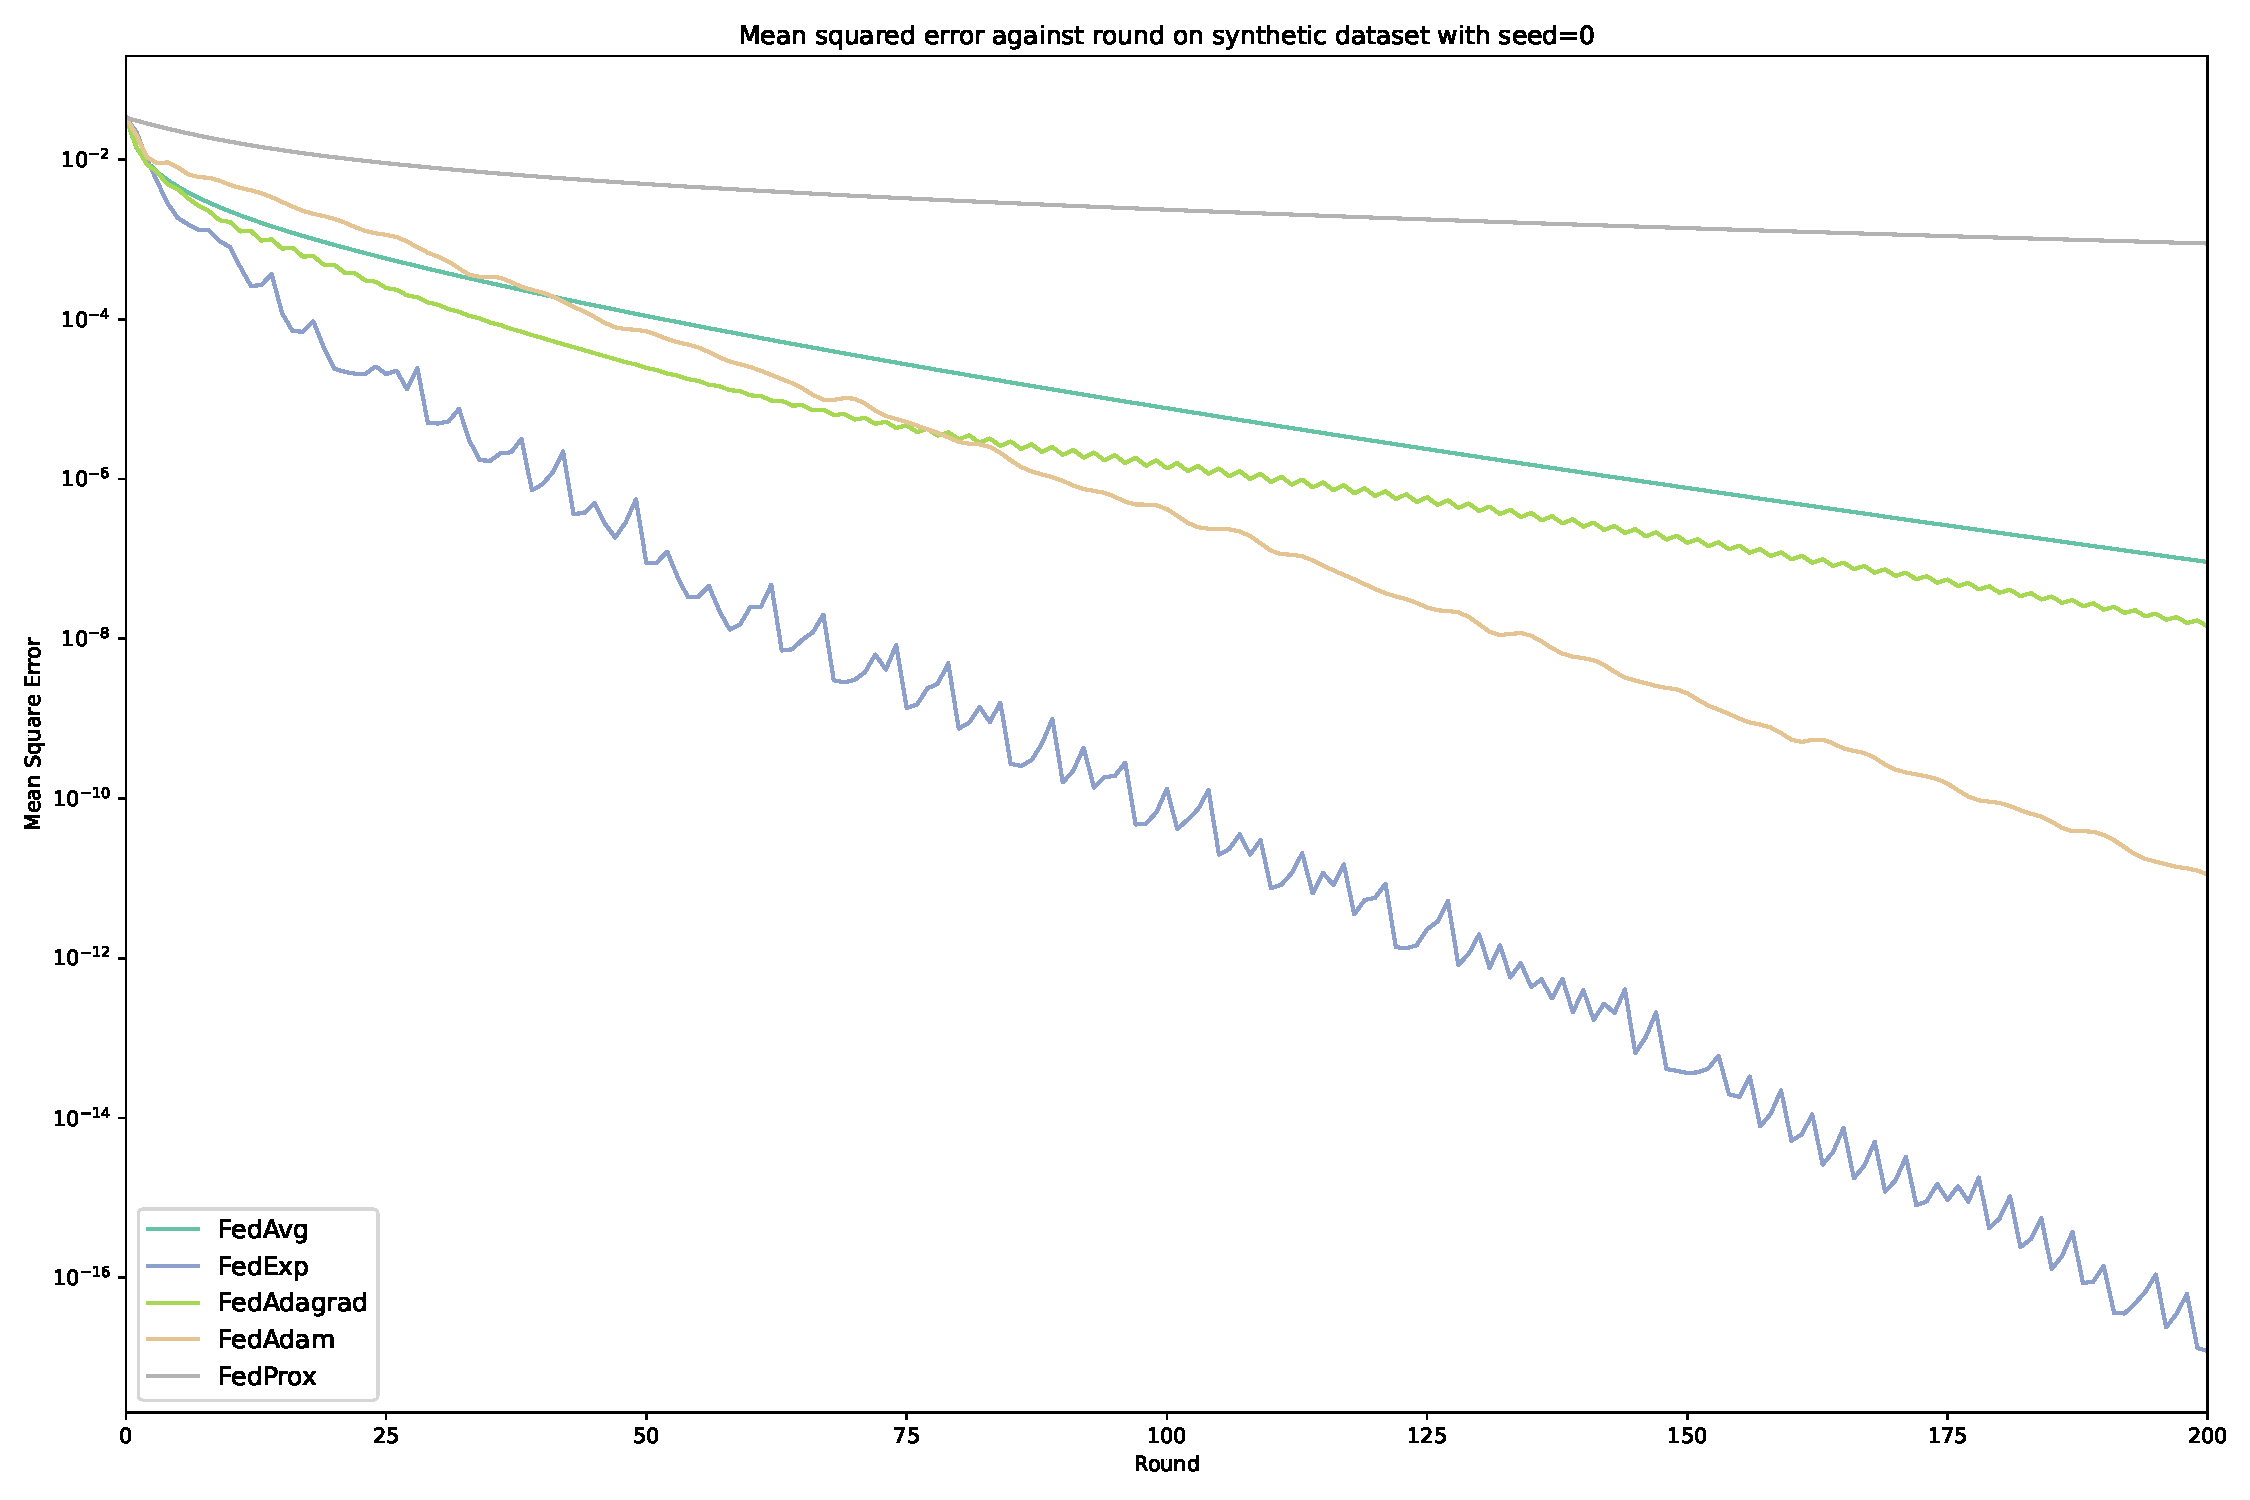
\includegraphics[width=.6\linewidth]{figs/syntheticSeed0_200Rounds.pdf}}
    \caption{Performance of different strategies on the synthetic data set, generated with np.random.seed(0)}
    \label{fig:200RoundsSeed0}
\end{figure}

\begin{figure}
    \centerline{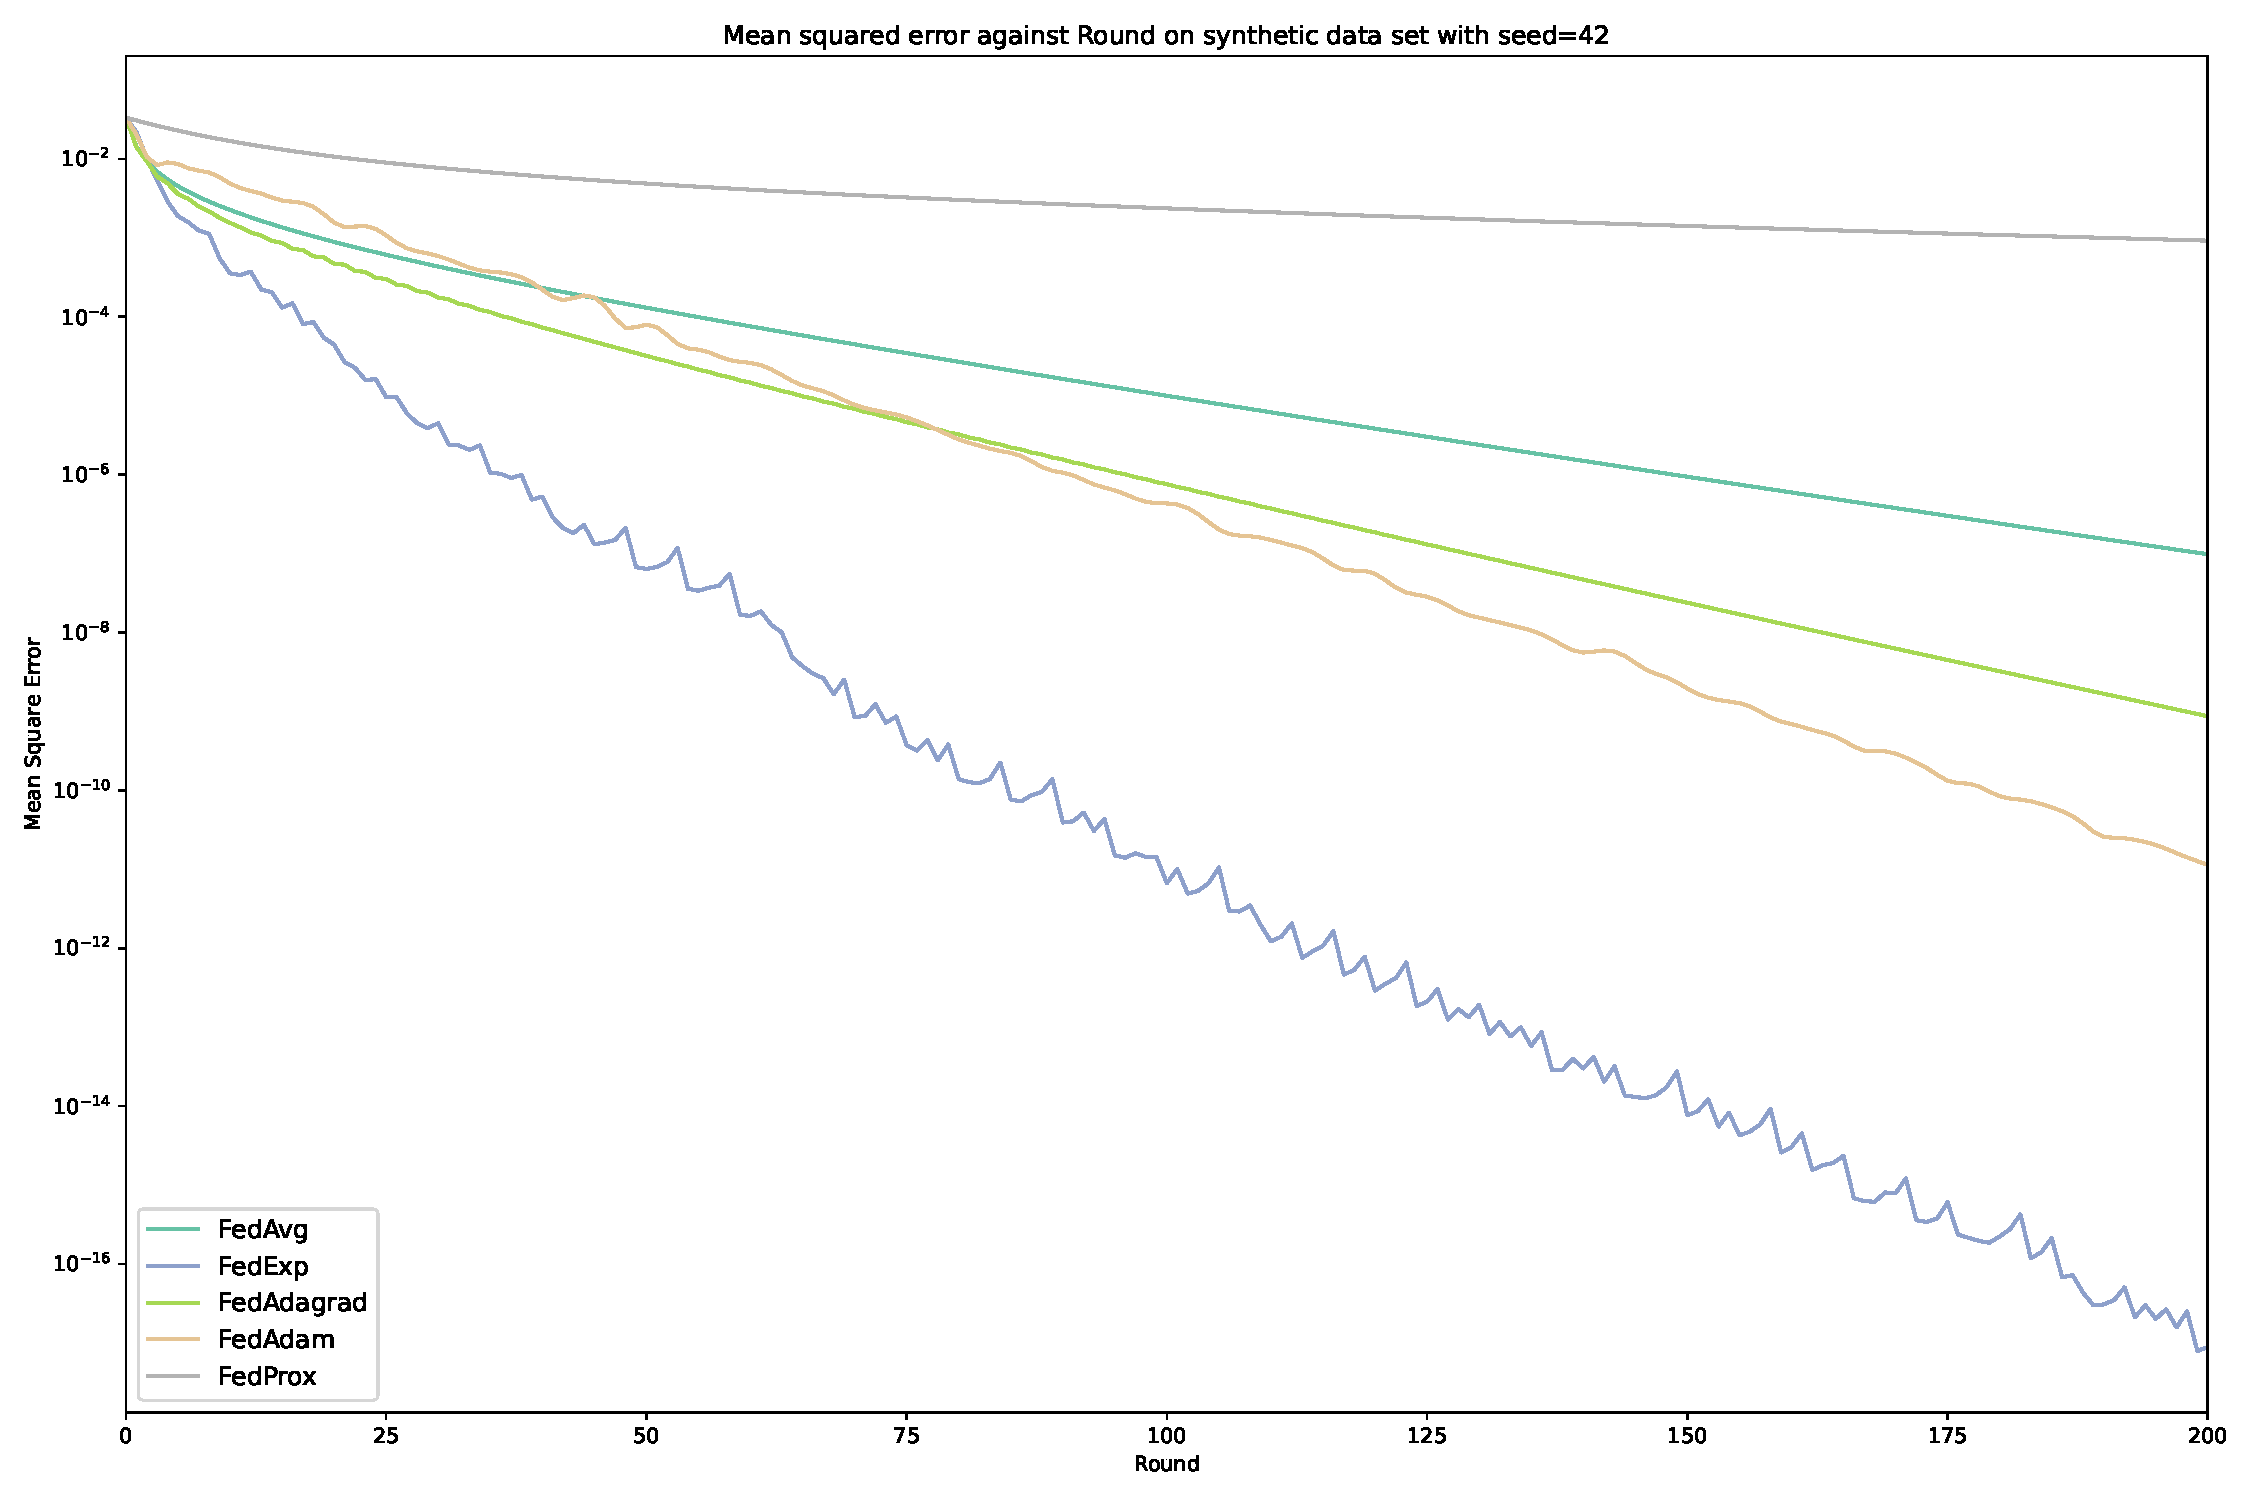
\includegraphics[width=.6\linewidth]{figs/syntheticSeed42_200Rounds.pdf}}
    \caption{Performance of different strategies on the synthetic data set, generated with np.random.seed(42)}
    \label{fig:200RoundsSeed42}
\end{figure}


\subsubsection{Effect of different number of rounds averaged over}

In figure \ref{fig:differentNumberOfAverageEvaluateRoundsSynthetic} the affect of changing the number of rounds which are averaged out to give the parameters for the evaluation.  As expected the larger the number of rounds averaged over the smoother the loss curve is.  The higher number of evaluation rounds all start their curves with very similar smooth curves, this is caused by the fact that the number of rounds is being increased on every extra round due to not actually having gone through all the rounds which is wanted to be averaged over.  This graph shows the clear trade off between having a much smoother curve and still having low loss, in the original paper they mention how increasing the number of rounds averaged over past 2 did not have much effect but we can see in the synthetic data set that it clearly does have a large effect, arguably 5 rounds looks to be the best trade off for this data set.  However in real data sets it is likely that their observations do hold and this higher number is caused by the very easy nature of the problem which is being solved. 

\begin{figure}
    \centerline{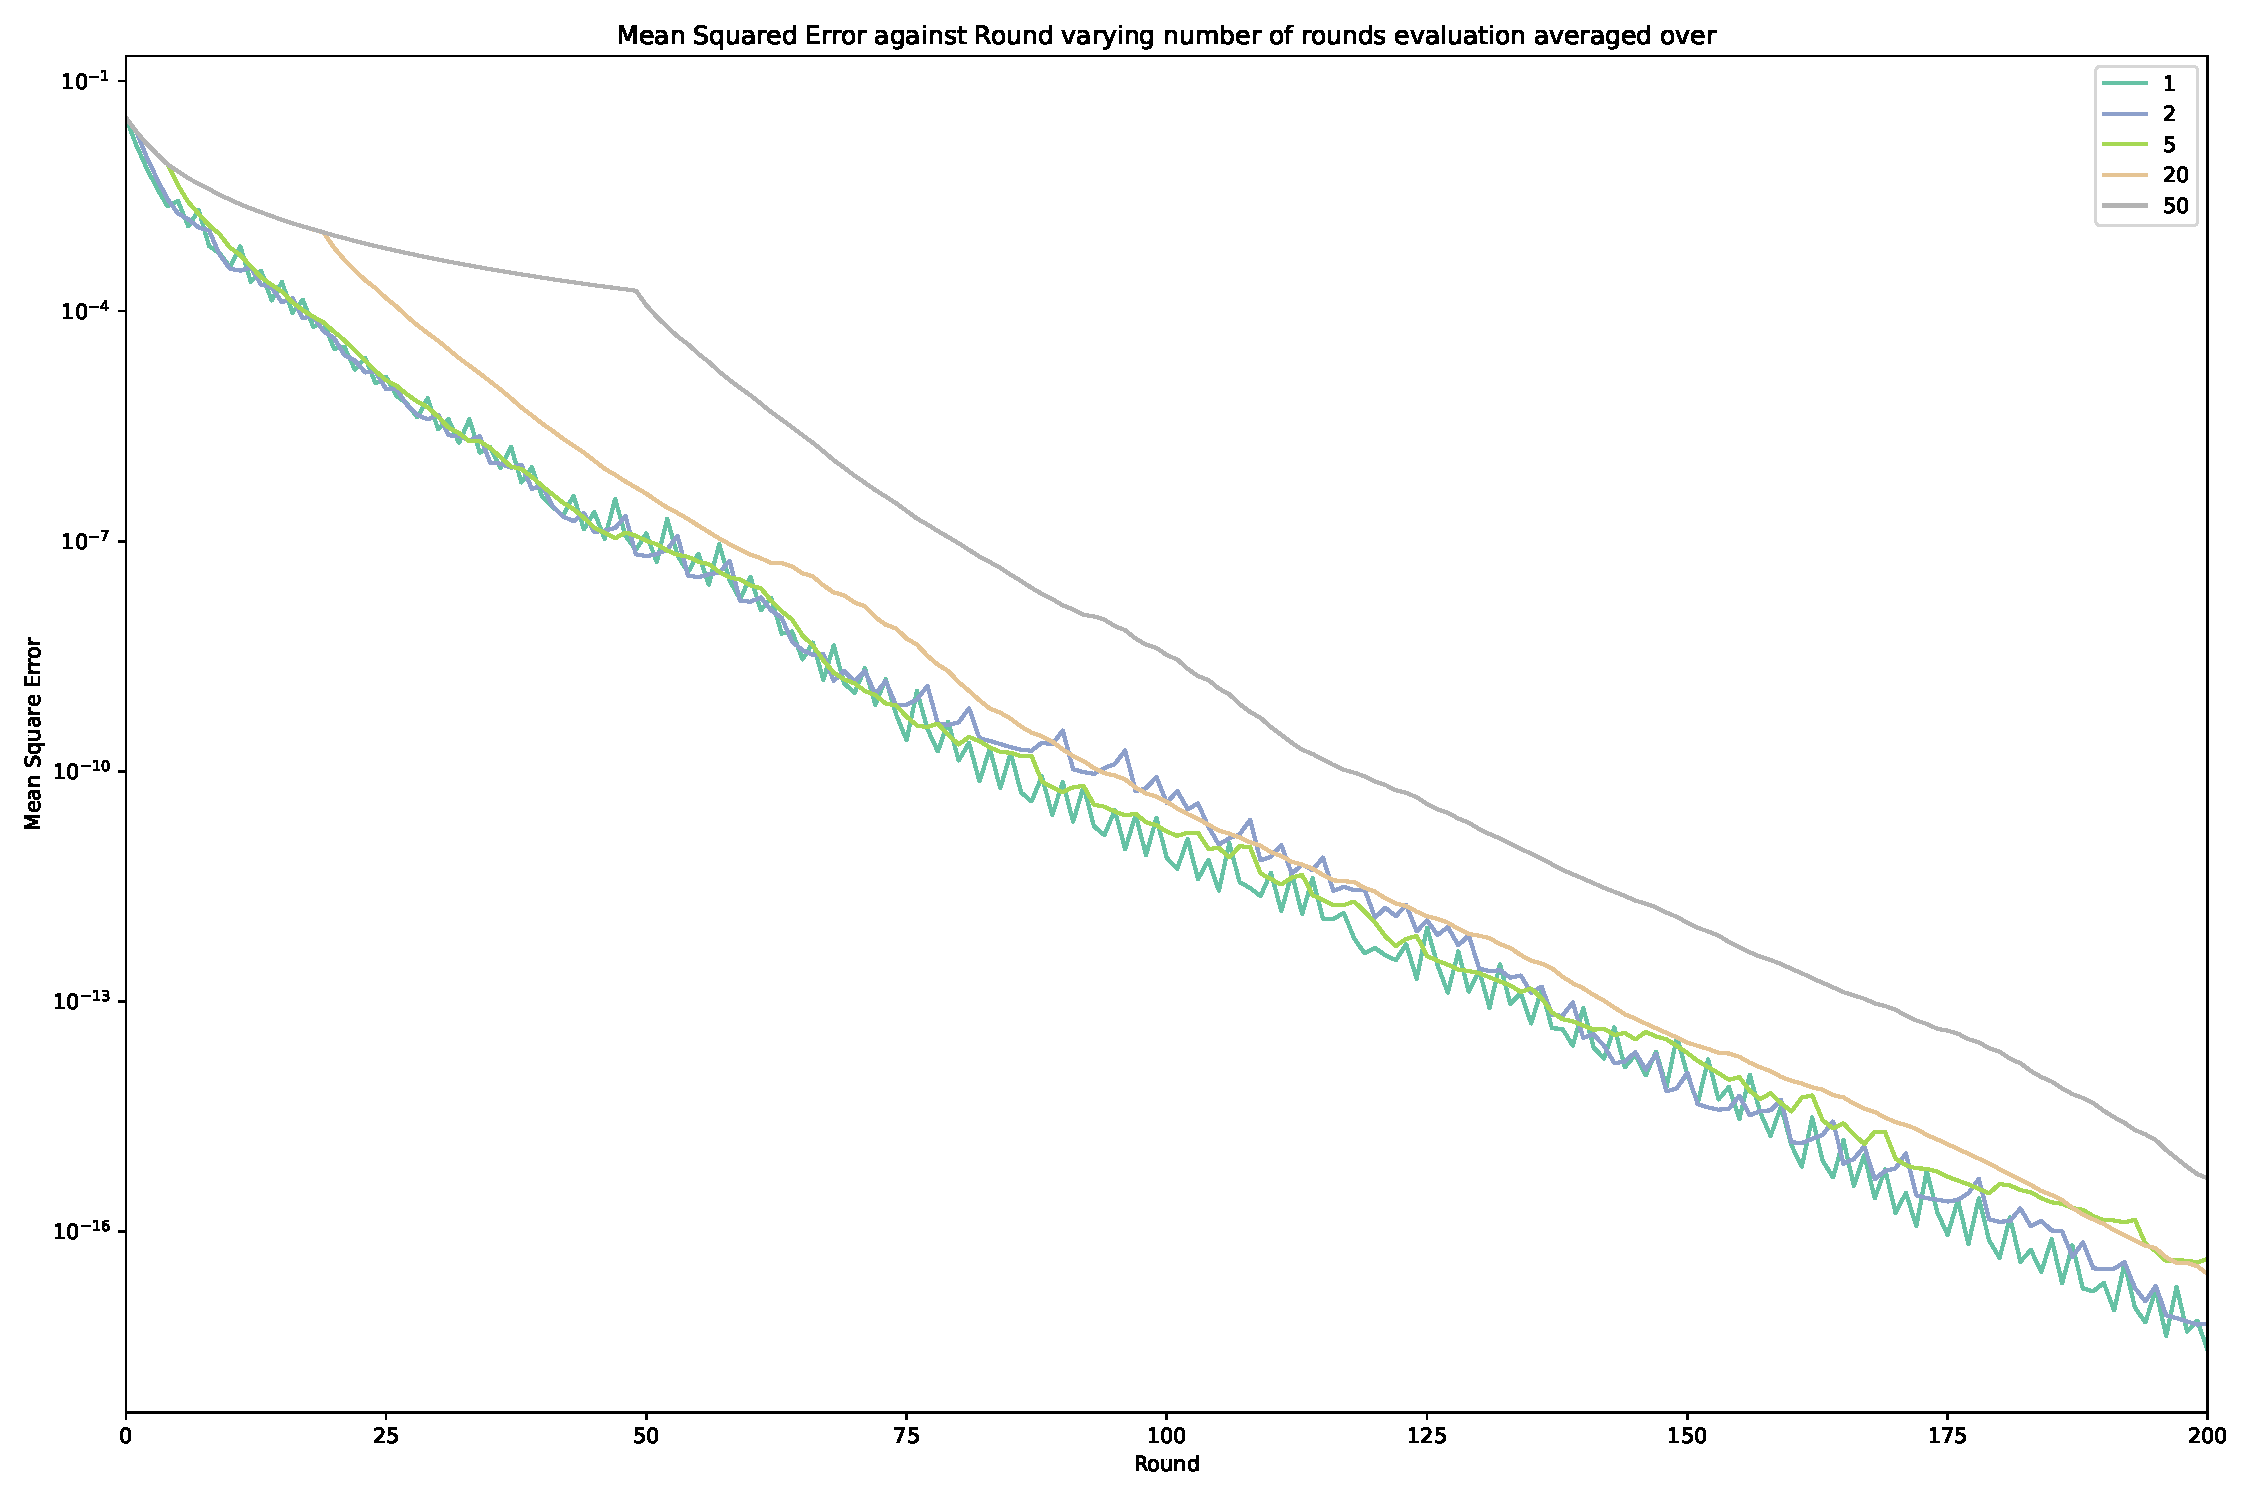
\includegraphics[width=.6\linewidth]{figs/synthetic_numberOfRoundsAverageEvaluate.pdf}}
    \caption{FedExP performance reported in evaluate averaging over different number of rounds}
    \label{fig:differentNumberOfAverageEvaluateRoundsSynthetic}
\end{figure}

\subsubsection{Long term behaviour}

In figure \ref{fig:2000RoundsSynthetic} the performance of the different strategies can be seen over a much larger number of rounds until the point that most of them are not improving any more.  FedProx is clearly the outlier, as before this is due to it having a much smaller global learning rate.  The performance of FedExP is quite interesting to observe because it clearly has the most perturbed loss curve when learning is actually happening but when it has learned the solution it has one of the smoothest curves; this makes sense from the algorithm because during the learning process it will have a very high global learning rate to make big changes but is able to lower the global learning rate dynamically to ensure that the weights are still getting closer to the optimal set of weights and can turn into FedAvg when the value suggested by extrapolation is small.  It is also clear from the graph that the end of performance of FedExP is actually higher than any other methods (although if run for a few thousand more rounds then it is likely that FedAvg would get very close), this shows that for this problem it is clearly the best strategy and has the good theoretical results in practice and that compared to other adaptive strategies it is not suffering from achieving a lower end performance compared with more simple strategies.

\begin{figure}
    \centerline{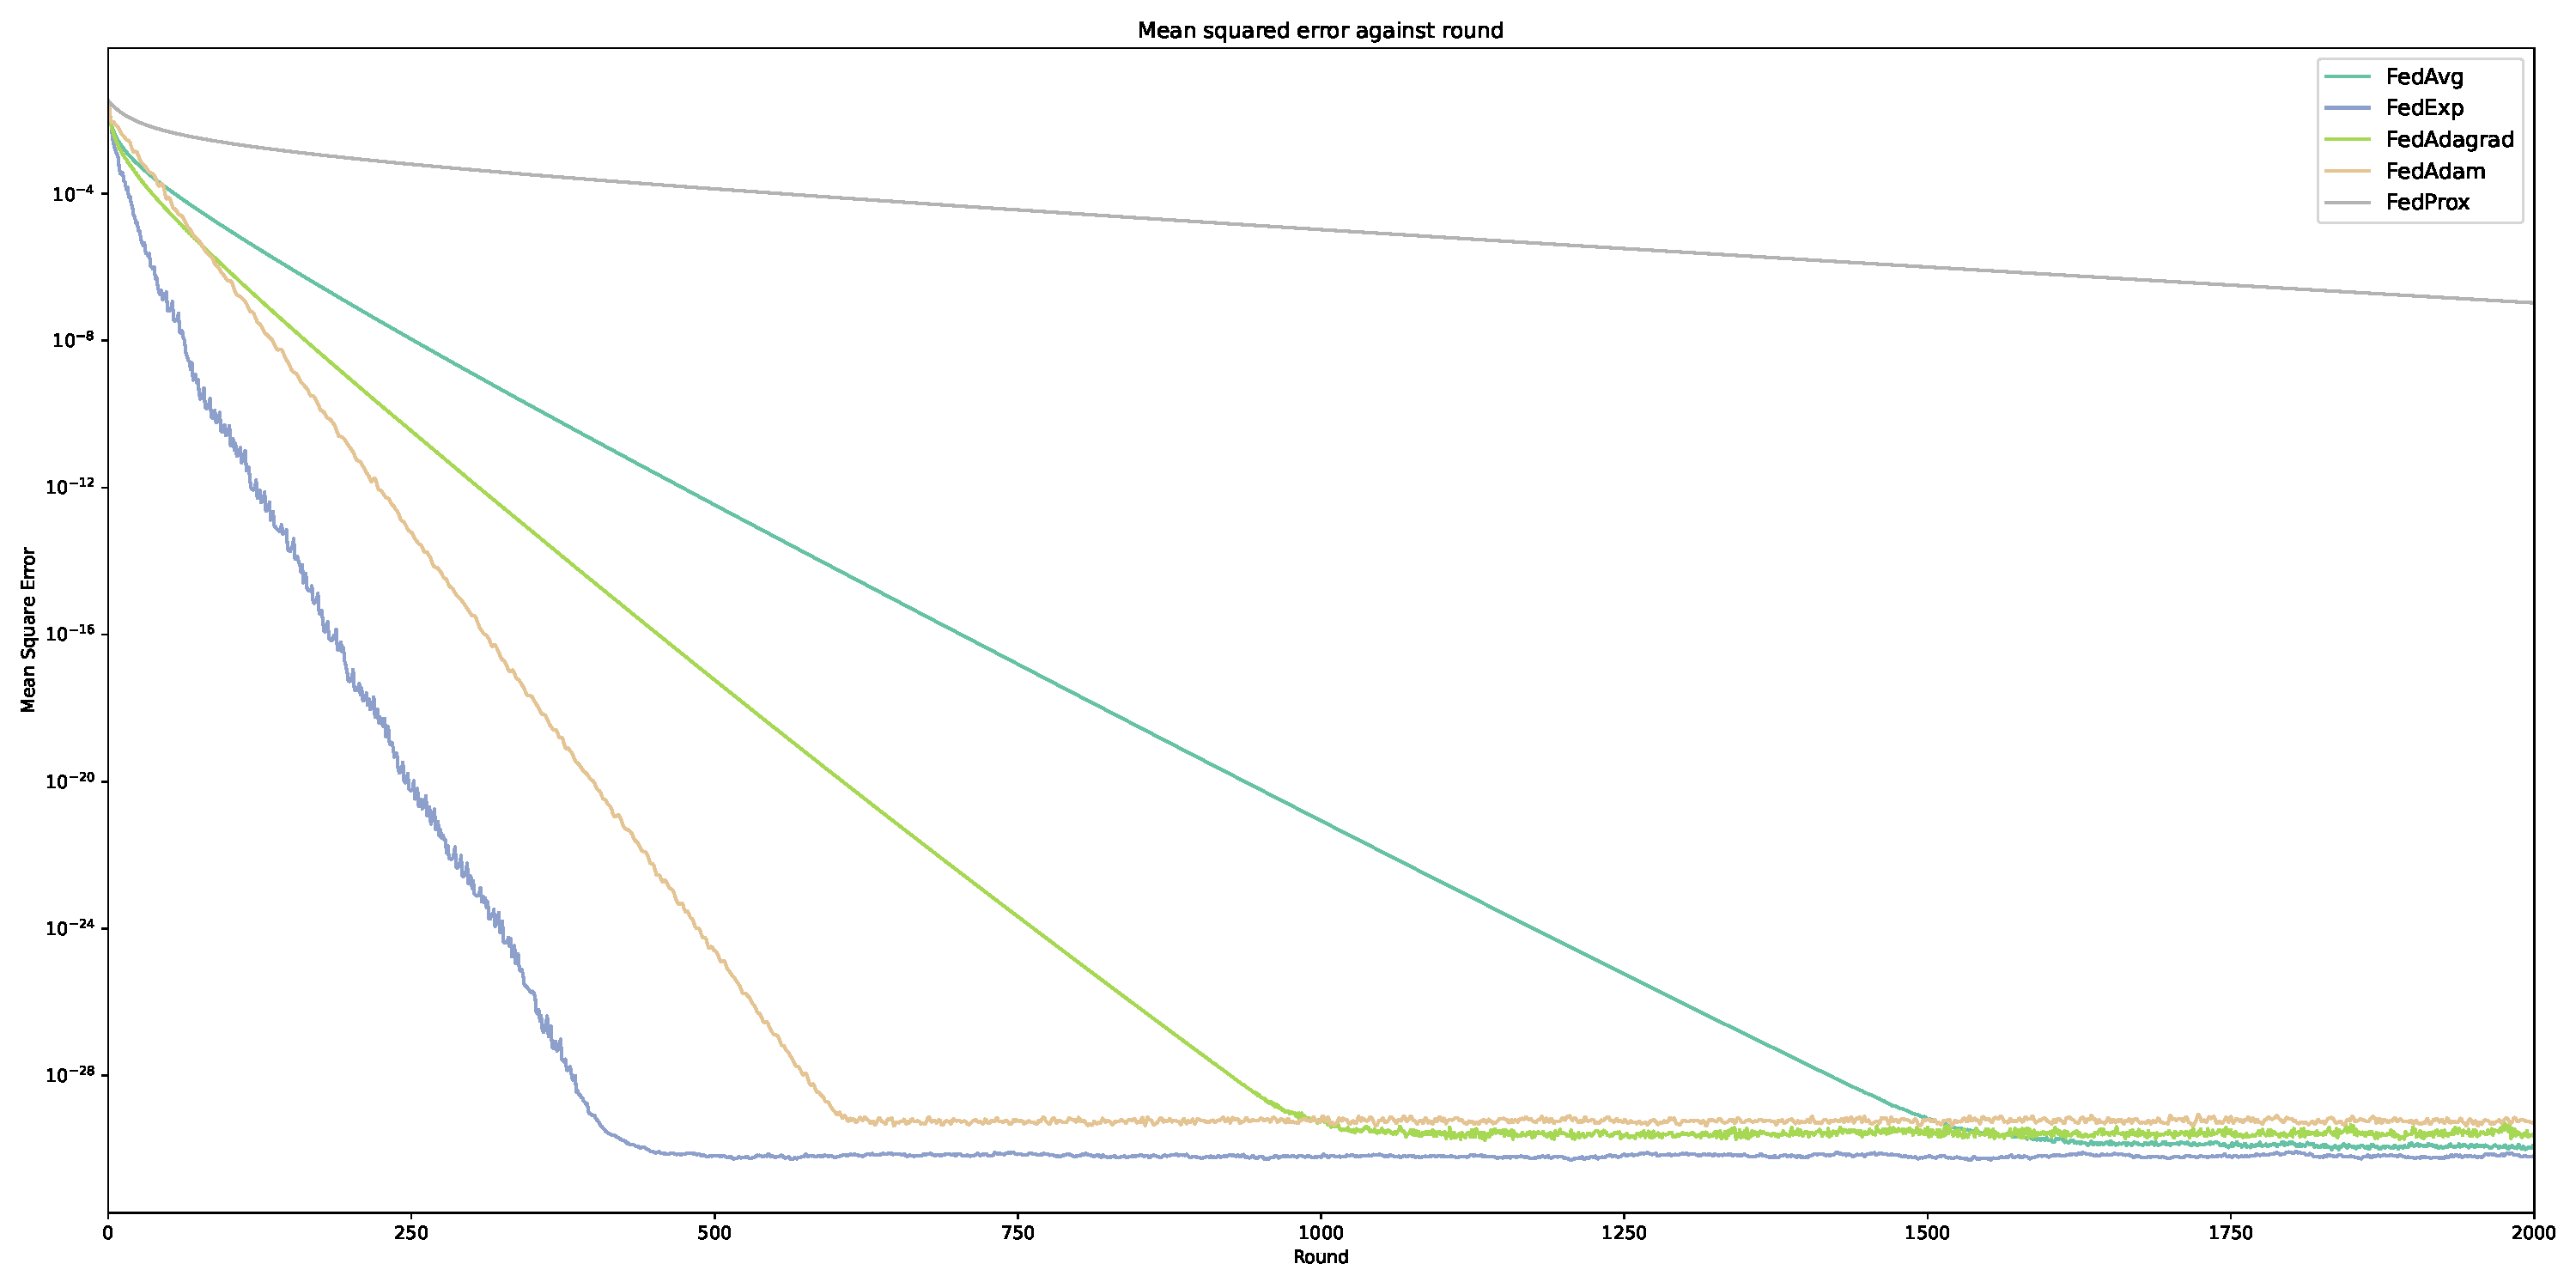
\includegraphics[width=\linewidth]{figs/synthetic_2000Rounds.pdf}}
    \caption{Performance of different strategies on the synthetic data set}
    \label{fig:2000RoundsSynthetic}
\end{figure}

\subsubsection{Varying $\epsilon$}

\begin{figure}
    \centerline{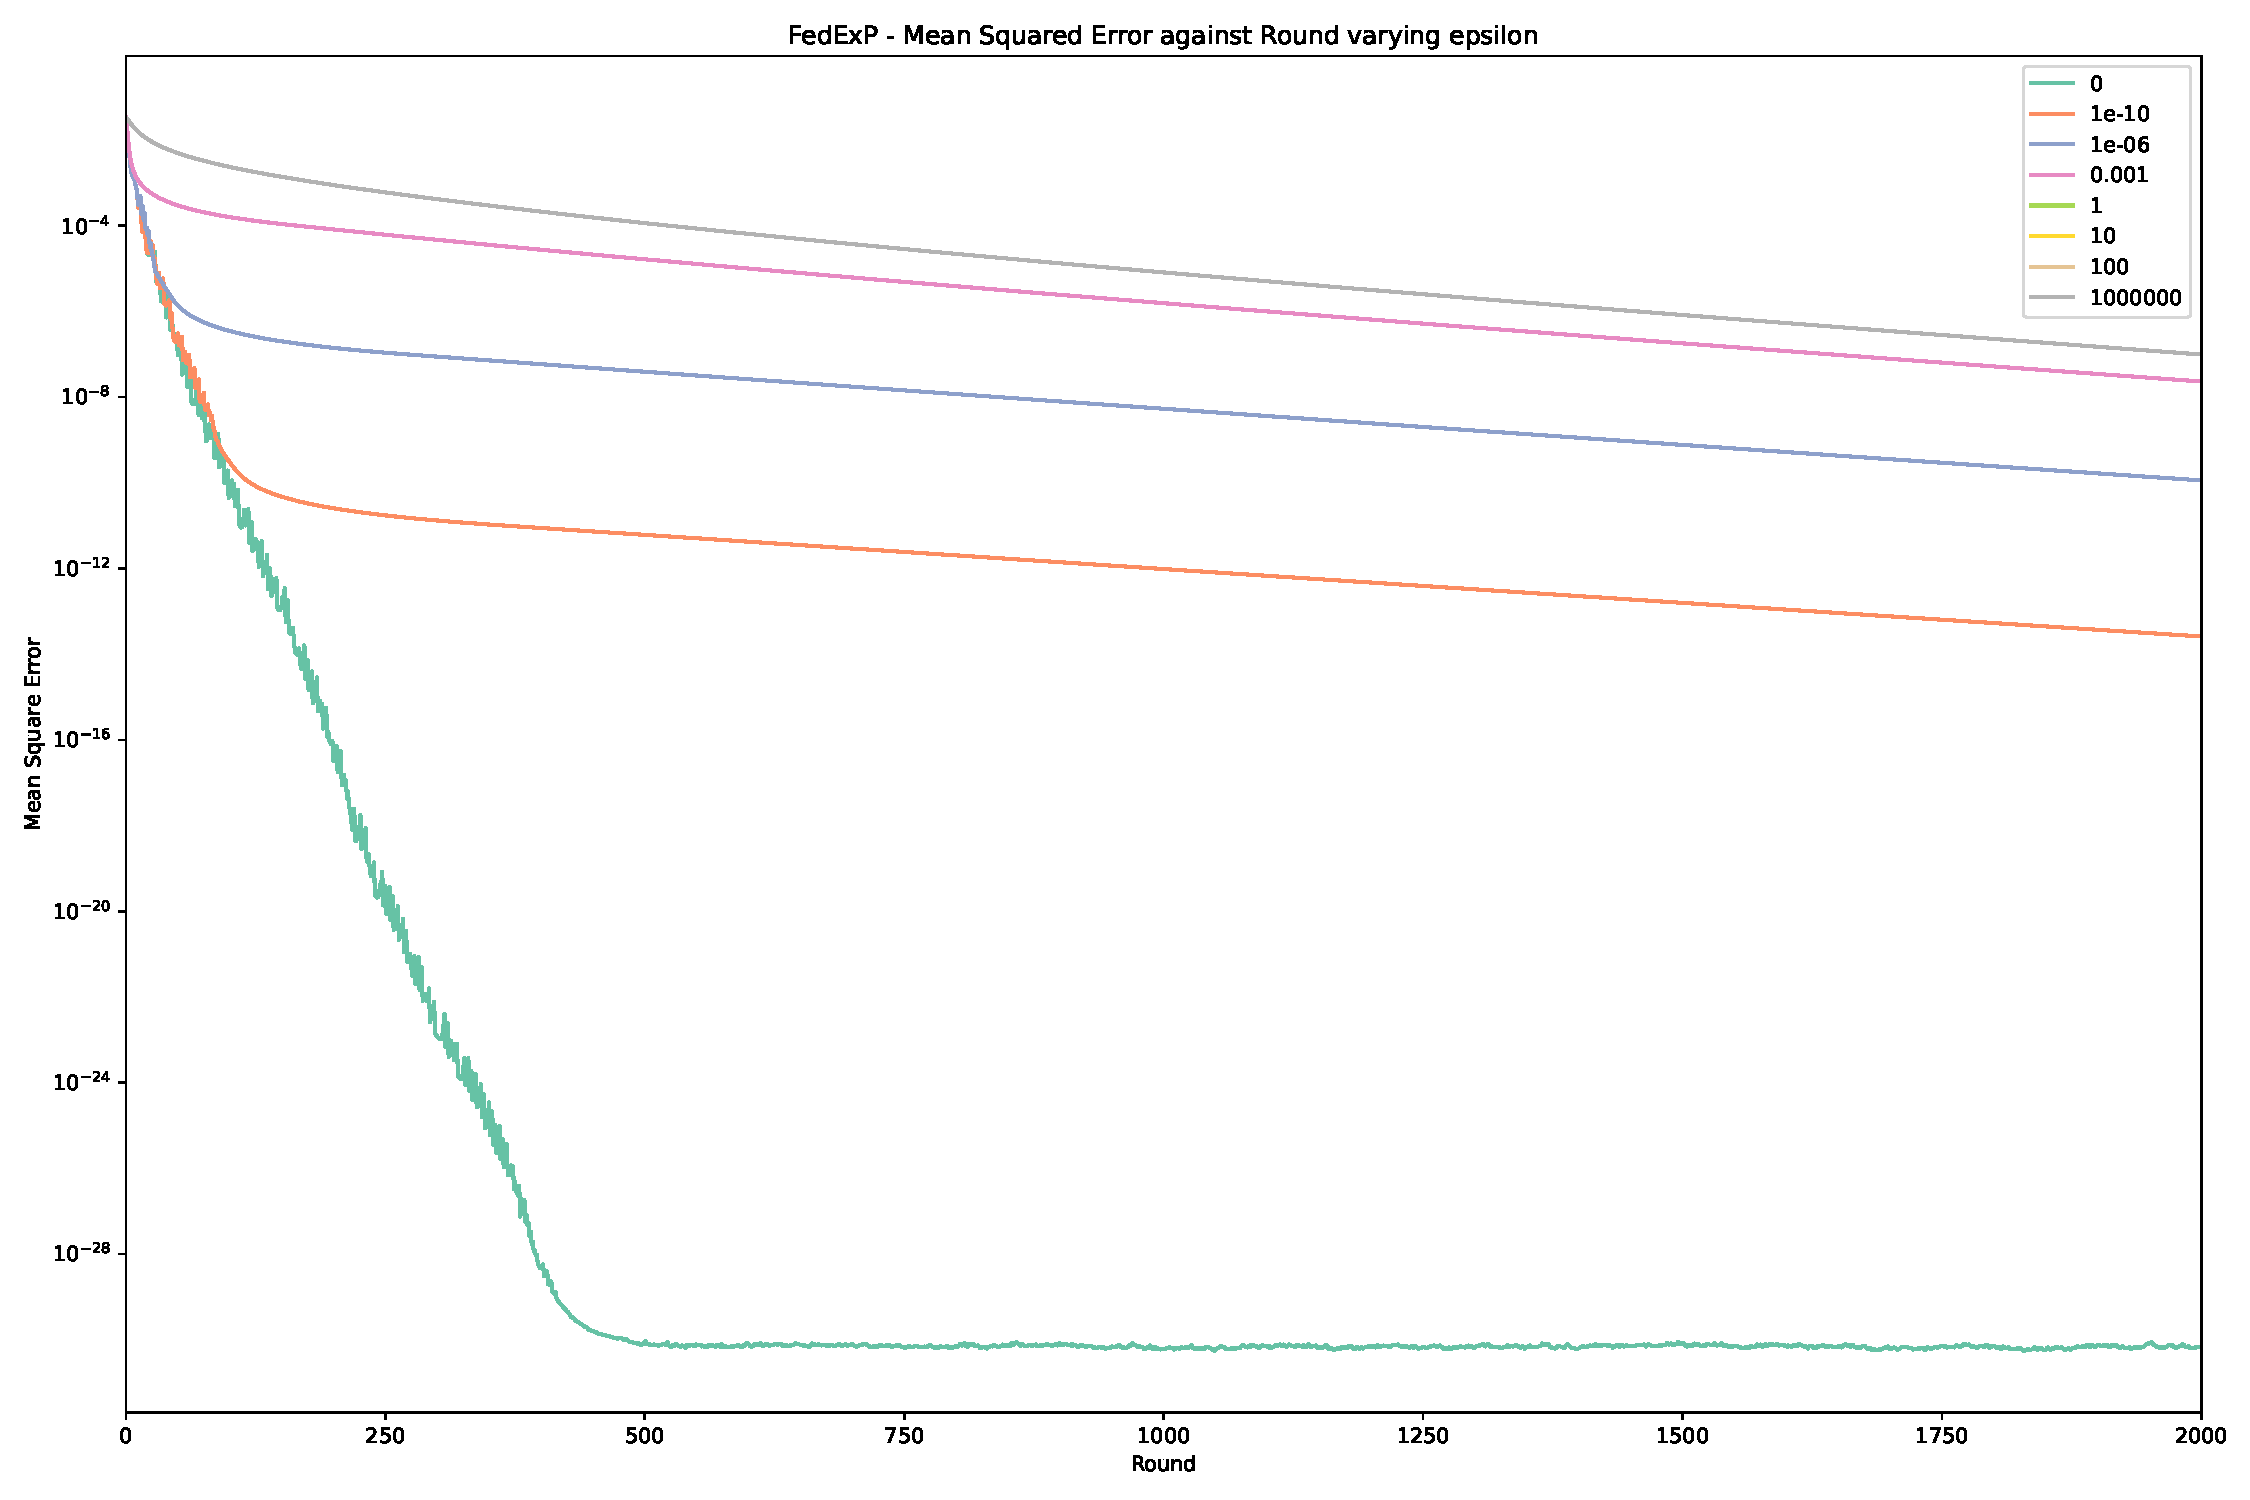
\includegraphics[width=.6\linewidth]{figs/synthetic_varyingEpsilon.pdf}}
    \caption{Performance of FedExP with varying $\epsilon$}
    \label{fig:varyingEpsilon}
\end{figure}

In figure \ref{fig:varyingEpsilon} the effects of changing the value of $\epsilon$ can be seen.  It is clear that having a higher value for $\epsilon$ leads to a smoother curve (because it is going to be using a smaller global learning rate therefore changes will not be as extreme to the overall model), while leading to significantly slower convergence to the optimal model.  The extreme sensitivity of performance to $\epsilon$ is likely to be a slight quirk of this data set, because the global learning rate chosen if not following the extrapolation is 1 but for the other strategies where the global learning rate is tuned it is set to 10, however the main point still stands in that increasing $\epsilon$ leads to performance closer to what FedAvg would achieve, it is also the case that above a certain point changing it has no effect because the extrapolation will never be chosen as the value for global learning rate.  The exact values of $\epsilon$ which should be chosen will depend on your model, due to that changing the size of the pseudo-gradient which is expected on each round, and the behaviour you want to see because if you want a smoother learning then a higher value will likely help but could slow down learning.  It is also possible that you would want to have an adaptive method for choosing the $\epsilon$ because as explained in the original paper it is mainly useful for when near convergence to the optimal solution, preventing massive learning rates caused by dividing a value very close to zero, therefore increasing it as you get closer could allow a good blending between the fast learning and smooth performance of FedAvg when near optimal solutions.

\subsection{Real data sets}

\begin{figure}
    \centerline{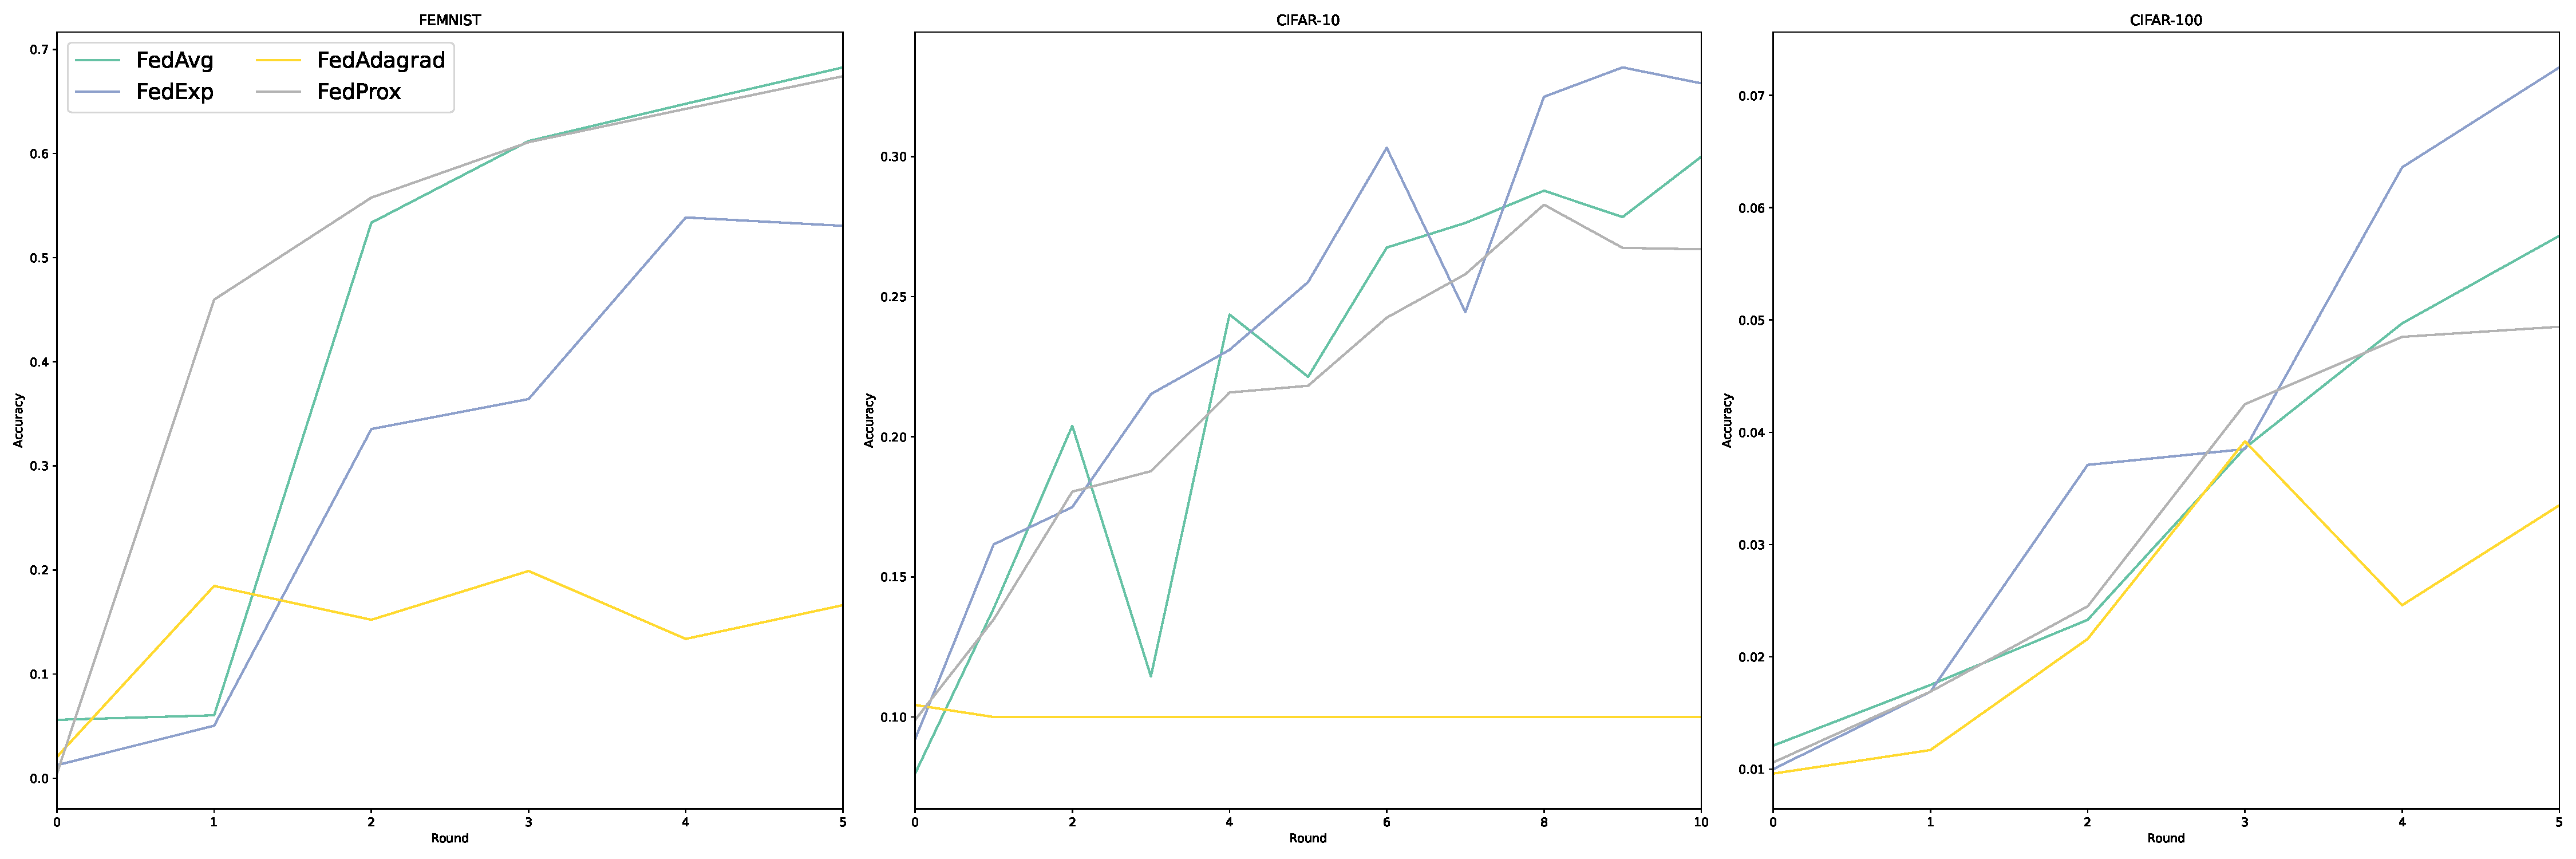
\includegraphics[width=\linewidth]{figs/realDatasetPerformance.pdf}}
    \caption{Performance of different strategies against real data sets}
    \label{fig:realDatasetPerformance}
\end{figure}

In figure \ref{fig:realDatasetPerformance} the performance of the different strategies initially is shown on several real data sets, we can see that FedExP is generally performing very well in comparison to the other strategies (for FEMNIST this does not look to hold but would likely be born out in longer runs); this is supported by what is shown in the paper where we expect FedExP to achieve faster convergence by dynamically selecting a good global learning rate.  The slight caveats to this are that FedAdagrad is not performing very well at all, this is likely due to mischosen hyper-parameters because of the differences between the FedAdagrad implementations explained above, and the settings for the CIFAR data sets differ to those in paper due to limited computational resources (only using 3 local epochs and 10 clients per round).

\subsubsection{FEMNIST Evaluate number of rounds}

In figure \ref{fig:femnistDifferentNumberOfEvaluateRounds} it is clear that the performance of FedExP is increased by averaging the weights used in evaluation compared to the raw weights, because we are following better global path, and that it has smaller perturbations in the loss curve getting closer to the performance of FedAvg.  This clearly show us that when working on real data sets it is important to average out several rounds of weights when evaluating the performance of the model, potentially more so than on the synthetic results because of the noticeably higher performance in this more difficult task.

\begin{figure}
    \centerline{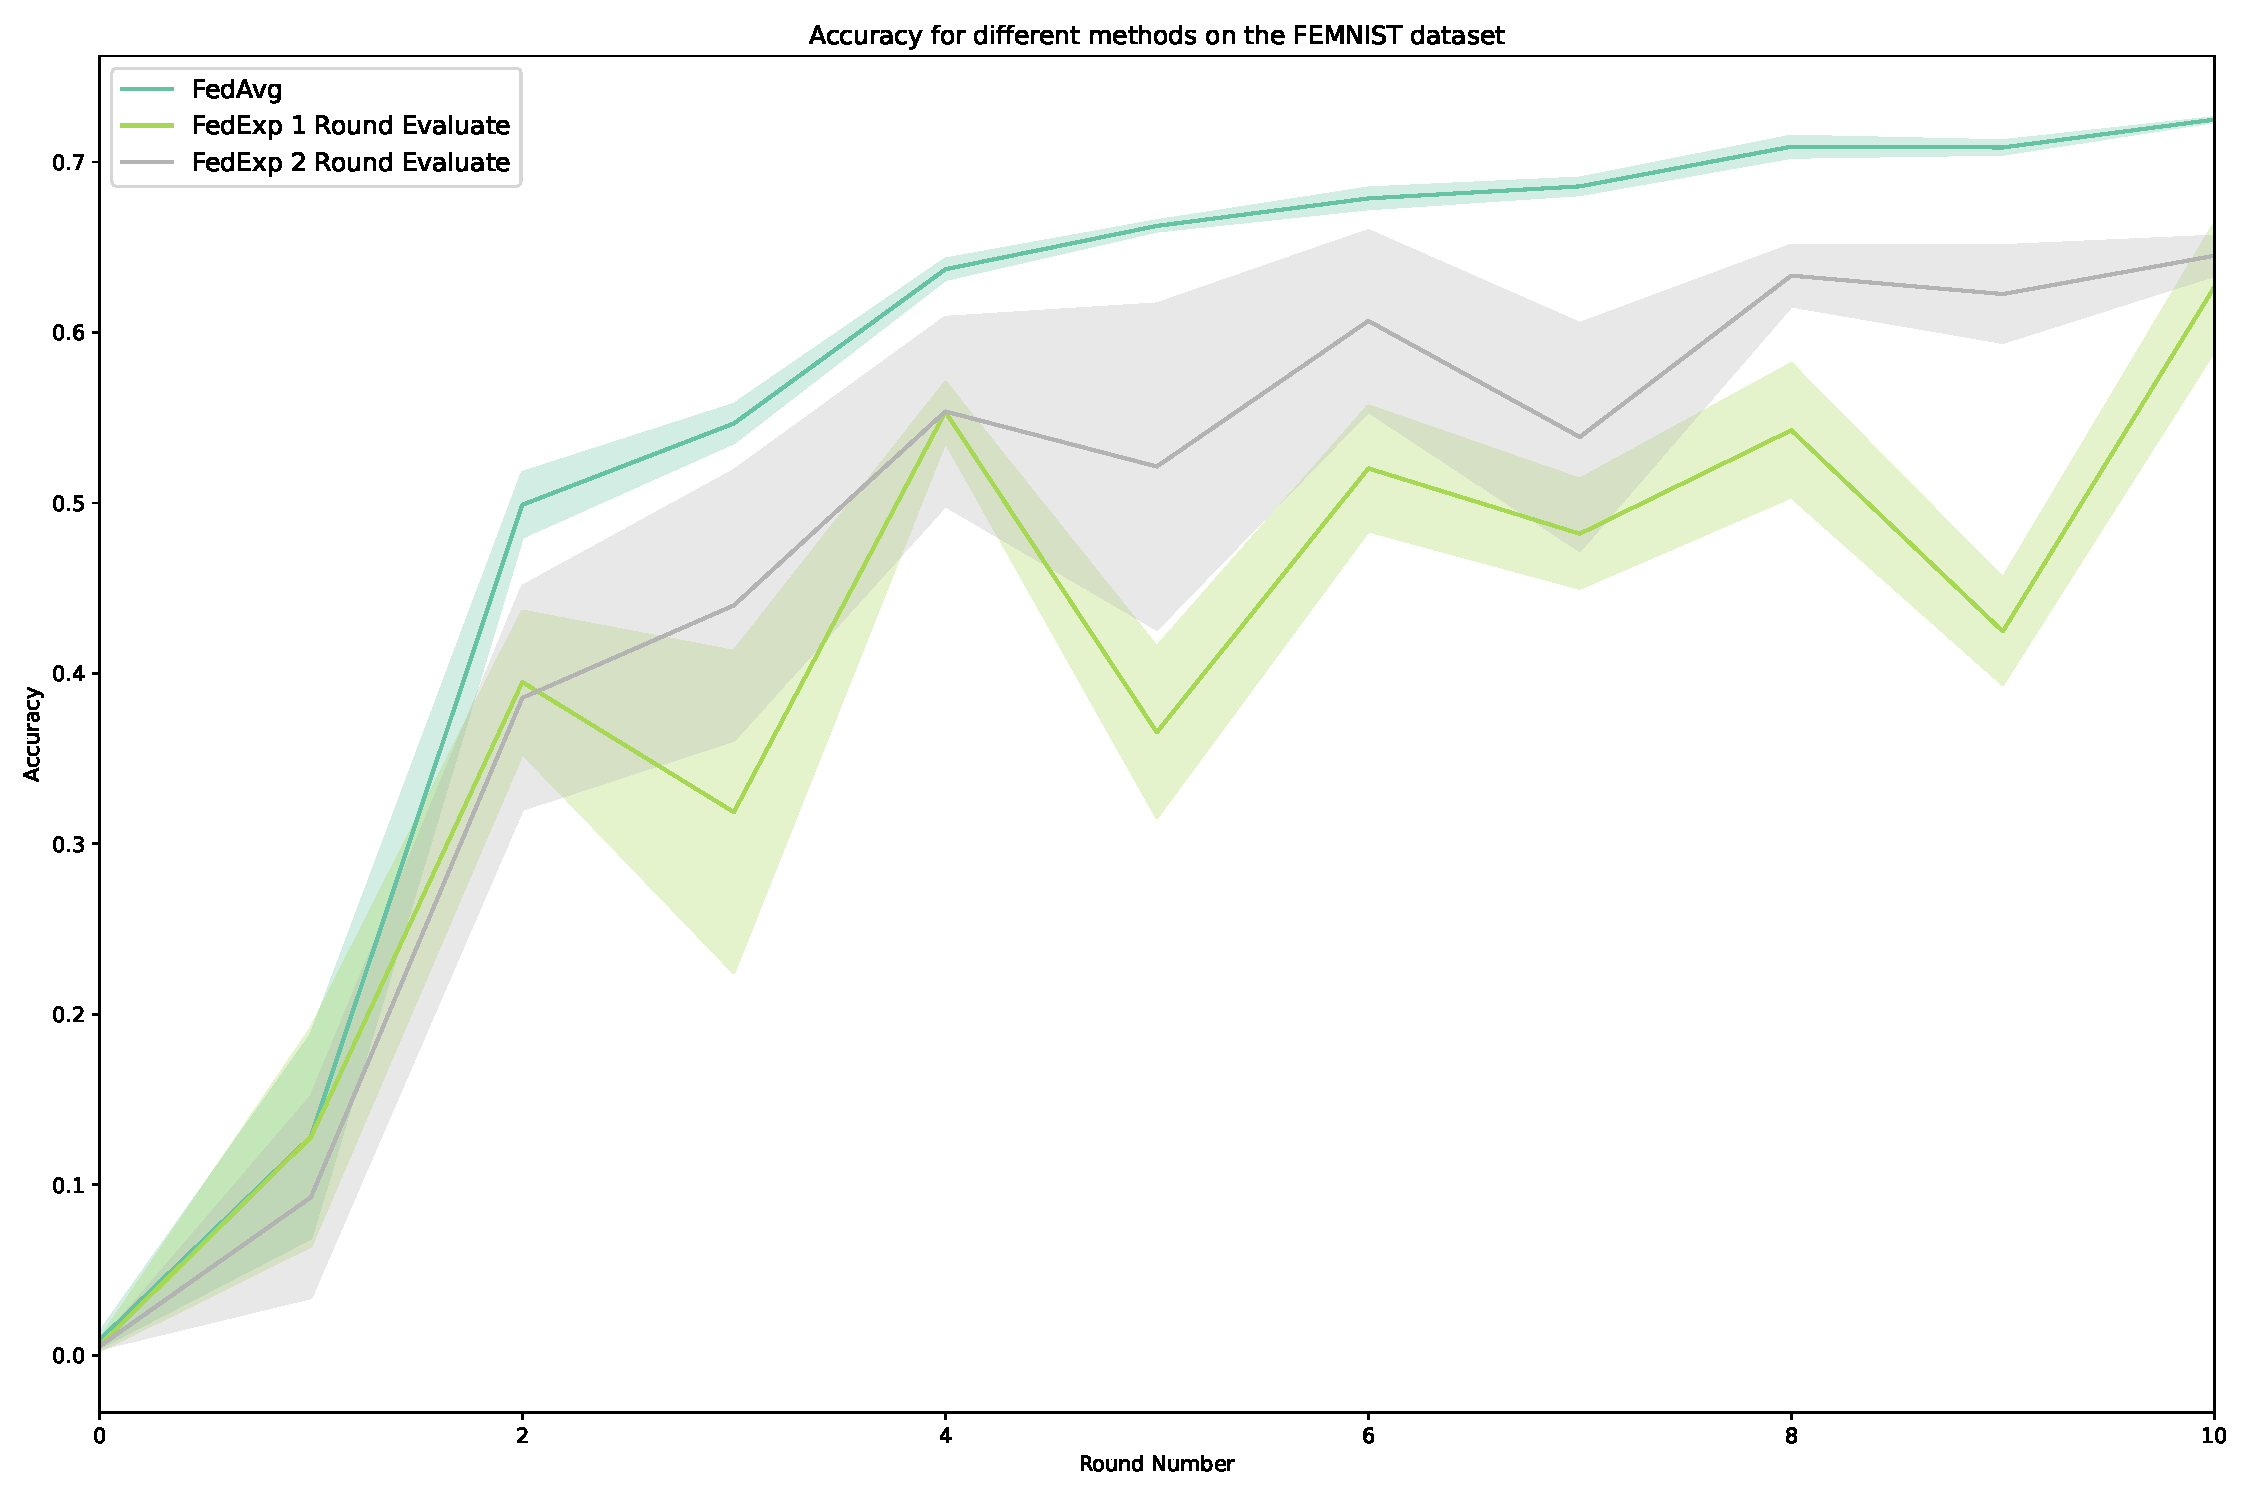
\includegraphics[width=.6\linewidth]{figs/femnist_fedexp_fedavg_evaluateRounds.pdf}}
    \caption{Performance of differing number of average rounds for FedExP against FedAvg on FEMNIST data set}
    \label{fig:femnistDifferentNumberOfEvaluateRounds}
\end{figure}

\section{Conclusion}

This project has successfully implemented the FedExP strategy into Flower and provided an analysis and comparison of its performance, with attention paid to how varying its hyper-parameters' change its behaviour.

\bibliography{refs}

\end{document}
